\chapter{GTFS}
\label{2-teorie-gtfs}

General Transit Feed Specification, zkráceně GTFS, je dokument, který definuje
obecný formát pro jízdní řády veřejné dopravy a příbuzné geografické informace.
GTFS „feeds“ umožňují veřejným dopravním agenturám zveřejňovat svá přepravní
data a vývojářům psát aplikace, které tato data spotřebovávají interoperabilním
způsobem. \cite{gtfs-info}

\section{Historie GTFS}
V Portlandu ve státě Oregon v USA se společnost TriMet pokusila jako jedna z prvních 
řešit problém s plánováním tranzitní dopravy pomocí otevřených dat sdílených širokou veřejností.
V roce 2005 společnost TriMet oslovila společnost Google s dotazem, zda mají nějaké plány
na začlenění tranzitní dopravy do svých plánovačů výletů na základě veřejných údajů TriMet.
Google jim kladně odpověděl a spojily síly s implementací jednoho z prvních plánovačů výletů v Portlandu.

Jedním z prvních problémů, kterým TriMet a Google čelily, byl problém udržitelných dat 
- pro zajištění kvalitních cest by plánovač cest potřeboval kvalitní přepravní řád, 
trasu a údaje o zastávkách v elektronickém formátu, který by byl neustále aktuální. 
Společnost TriMet ve spolupráci se společností Google naformátovala svá přepravní 
data do snadno udržovatelného a spotřebního formátu, který lze importovat do Map Google. 
Tento formát dat přepravy se stal známým jako Specifikace zdroje Google Transit (anglicky
Google Transit Feed Specification (GTFS)). 
V roce 2005 byla tato služba plánování cesty spuštěna jako Google Transit.

Od tohoto roku se GTFS stal nejpopulárnějším datovým formátem pro přepravní služby na světě. 
Spousta agentur se rozhodla sdílet své GTFS údaje s veřejností, zatímco některé agentury 
zůstaly zdrženlivé a přístup k datům nechaly jen některým partnerům. Ke 2. prosinci 2019
uvádí OpenMobilityData 1233 poskytovatelů s veřejně přístupnými kanály GTFS,
z nichž 465 je ve Spojených státech. 

V důsledku inovací vývojářů třetích stran jsou data GTFS nyní využívána různými softwarovými aplikacemi
třetích stran k mnoha různým účelům, včetně plánování výletů, map, vytváření jízdních řádů, mobilních dat,
vizualizace, přístupnosti, analytických nástrojů pro plánování a informační systémy v reálném čase.
V roce 2010 byl název formátu GTFS změněn na General Transit Feed Specification,
aby přesně reprezentoval jeho použití v mnoha různých aplikacích mimo produkty Google. \cite{transitwiki} 

% doplnit něco o historii GTFS 

\section{GTFS dataset}
GTFS "feed" nebo lépe jako GTFS dataset\footnote{kolekce dat, která by měla být publikována na permanantní URL adrese}
je ZIP soubor, který obsahuje CSV soubory.

CSV, \textit{Comma-separated values}, v překladu \textit{hodnoty oddělené čárkami}, je jednoduchý 
souborový formát určený pro výměnu tabulkových dat. Data jsou oddělována „oddělovačem“.
Ačkoli podle definice by měl být formát oddělen čárkami, oddělovač může být prakticky cokoli. 
Nejčastějšími oddělovači jsou právě čárky, středníky nebo mezery. CSV soubor se 
může upravovat v jakémkoliv textovém editoru.

\begin{figure}[H] \centering
    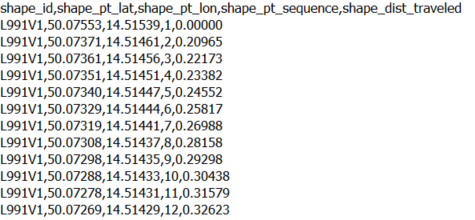
\includegraphics[width=250pt]{./pictures/ukazka-csv.PNG}
    \caption[Ukázka CSV formátu ze souboru shapes.txt]{Ukázka CSV formátu ze souboru shapes.txt}
	\label{fig:ukazka-csv}              
\end{figure}

V GTFS datasetu může být v současné době až 17 CSV souborů v textové podobě. Slovem "může" je myšleno to,
že některé CSV soubory jsou požadované či podmíněně požadované a jiné volitelné.
Jaké CSV soubory soubory obsahuje dataset záleží na konkrétním dopravním systému, který
tento dataset vytváří.

Termín "požadované" znamená, že daný CSV soubor se musí nacházet v GTFS datasetu nebo dané pole
se musí nacházet v CSV souboru a v tomto poli musí být uvedena hodnota pro každý záznam. 

%přidat referenci na podmínky?
Termín "podmíněně požadované" znamená, že daný CSV soubor nebo pole je vyžadován za určitých podmínek, 
které jsou uvedeny v popisu souboru nebo pole. Mimo tyto podmínky je tento soubor nebo pole volitelný.

Termín "volitelné" znamená, že daný CSV soubor nebo pole může být vynecháno. V případě zahrnutí 
volitelného sloupec, mohou být některé položky v tomto poli prázdné řetězce, což je ekvivalentní s prázdným
polem.

V následující tabulce \ref{table:csv-soubory} jsou přehledně zobrazeny všechny CSV soubory,
které v současnosti v GTFS datasetu mohou být.

\newcolumntype{s}{>{\centering\arraybackslash\columncolor[HTML]{CCFFCC}} m{5cm}}
\newcolumntype{v}{>{\centering\arraybackslash\columncolor[HTML]{C4FFFD}} m{5cm}}

\begin{table}[h!]
\begin{center}
\begin{tabular}{ |s|v| } 
  \hline
  požadované/podmíněně požadované & volitelné \\ 
  \hline
  agency.txt & fare\_attributes.txt \\ 
  stops.txt & fare\_rules.txt \\ 
  routes.txt & shapes.txt \\
  trips.txt & frequencies.txt \\
  stop\_times.txt & transfers.txt \\
  calendar.txt & pathways.txt \\
  calendar\_dates.txt & levels.txt \\ 
  feed\_info.txt & translations.txt \\
  - & attributions.txt \\ 
  \hline      
\end{tabular}
\end{center}
\caption{Seznam CSV souborů v GTFS datasetu}
\label{table:csv-soubory}
\end{table}

Každý CSV soubor v GTFS datasetu má v prvním řádku názvy polí, do kterých je tento
soubor rozřazen. Jednotlivá pole mají různý datový typ, která jsou barva, kód měny, 
datum, email, enum (výčet), ID, kód jazyka, zeměpisná délka, zeměpisná šířka,
nezáporné číslo s plovoucí desetinnou čárkou, nezáporné celé číslo, telefonní číslo,
čas, text, časové pásmo a URL adresa.

Jedno z nejdůležitějších polí je pole s datovým typem ID, což je hodnota jednoznačně určuje každý záznam.
Právě tento datový typ umožňuje propojení jednotlivých CSV souborů mezi sebou. ID může být
sekvence libovolných UTF-8 znaků. Pole s datovým typem ID se označují nakonci názvu s 
"\_id". Na následujícím obrázku \ref{fig:GTFS-diagram} je toto propojení zobrazeno pomocí diagramů.

%přidat referenci na podmínky?
Na obrázku \ref{fig:GTFS-diagram} je taktéž tučně zobrazeno, které pole jsou v daném CSV souboru
jsou požadované, podmíněně požadované nebo volitelné. 

\begin{figure}[H] \centering
    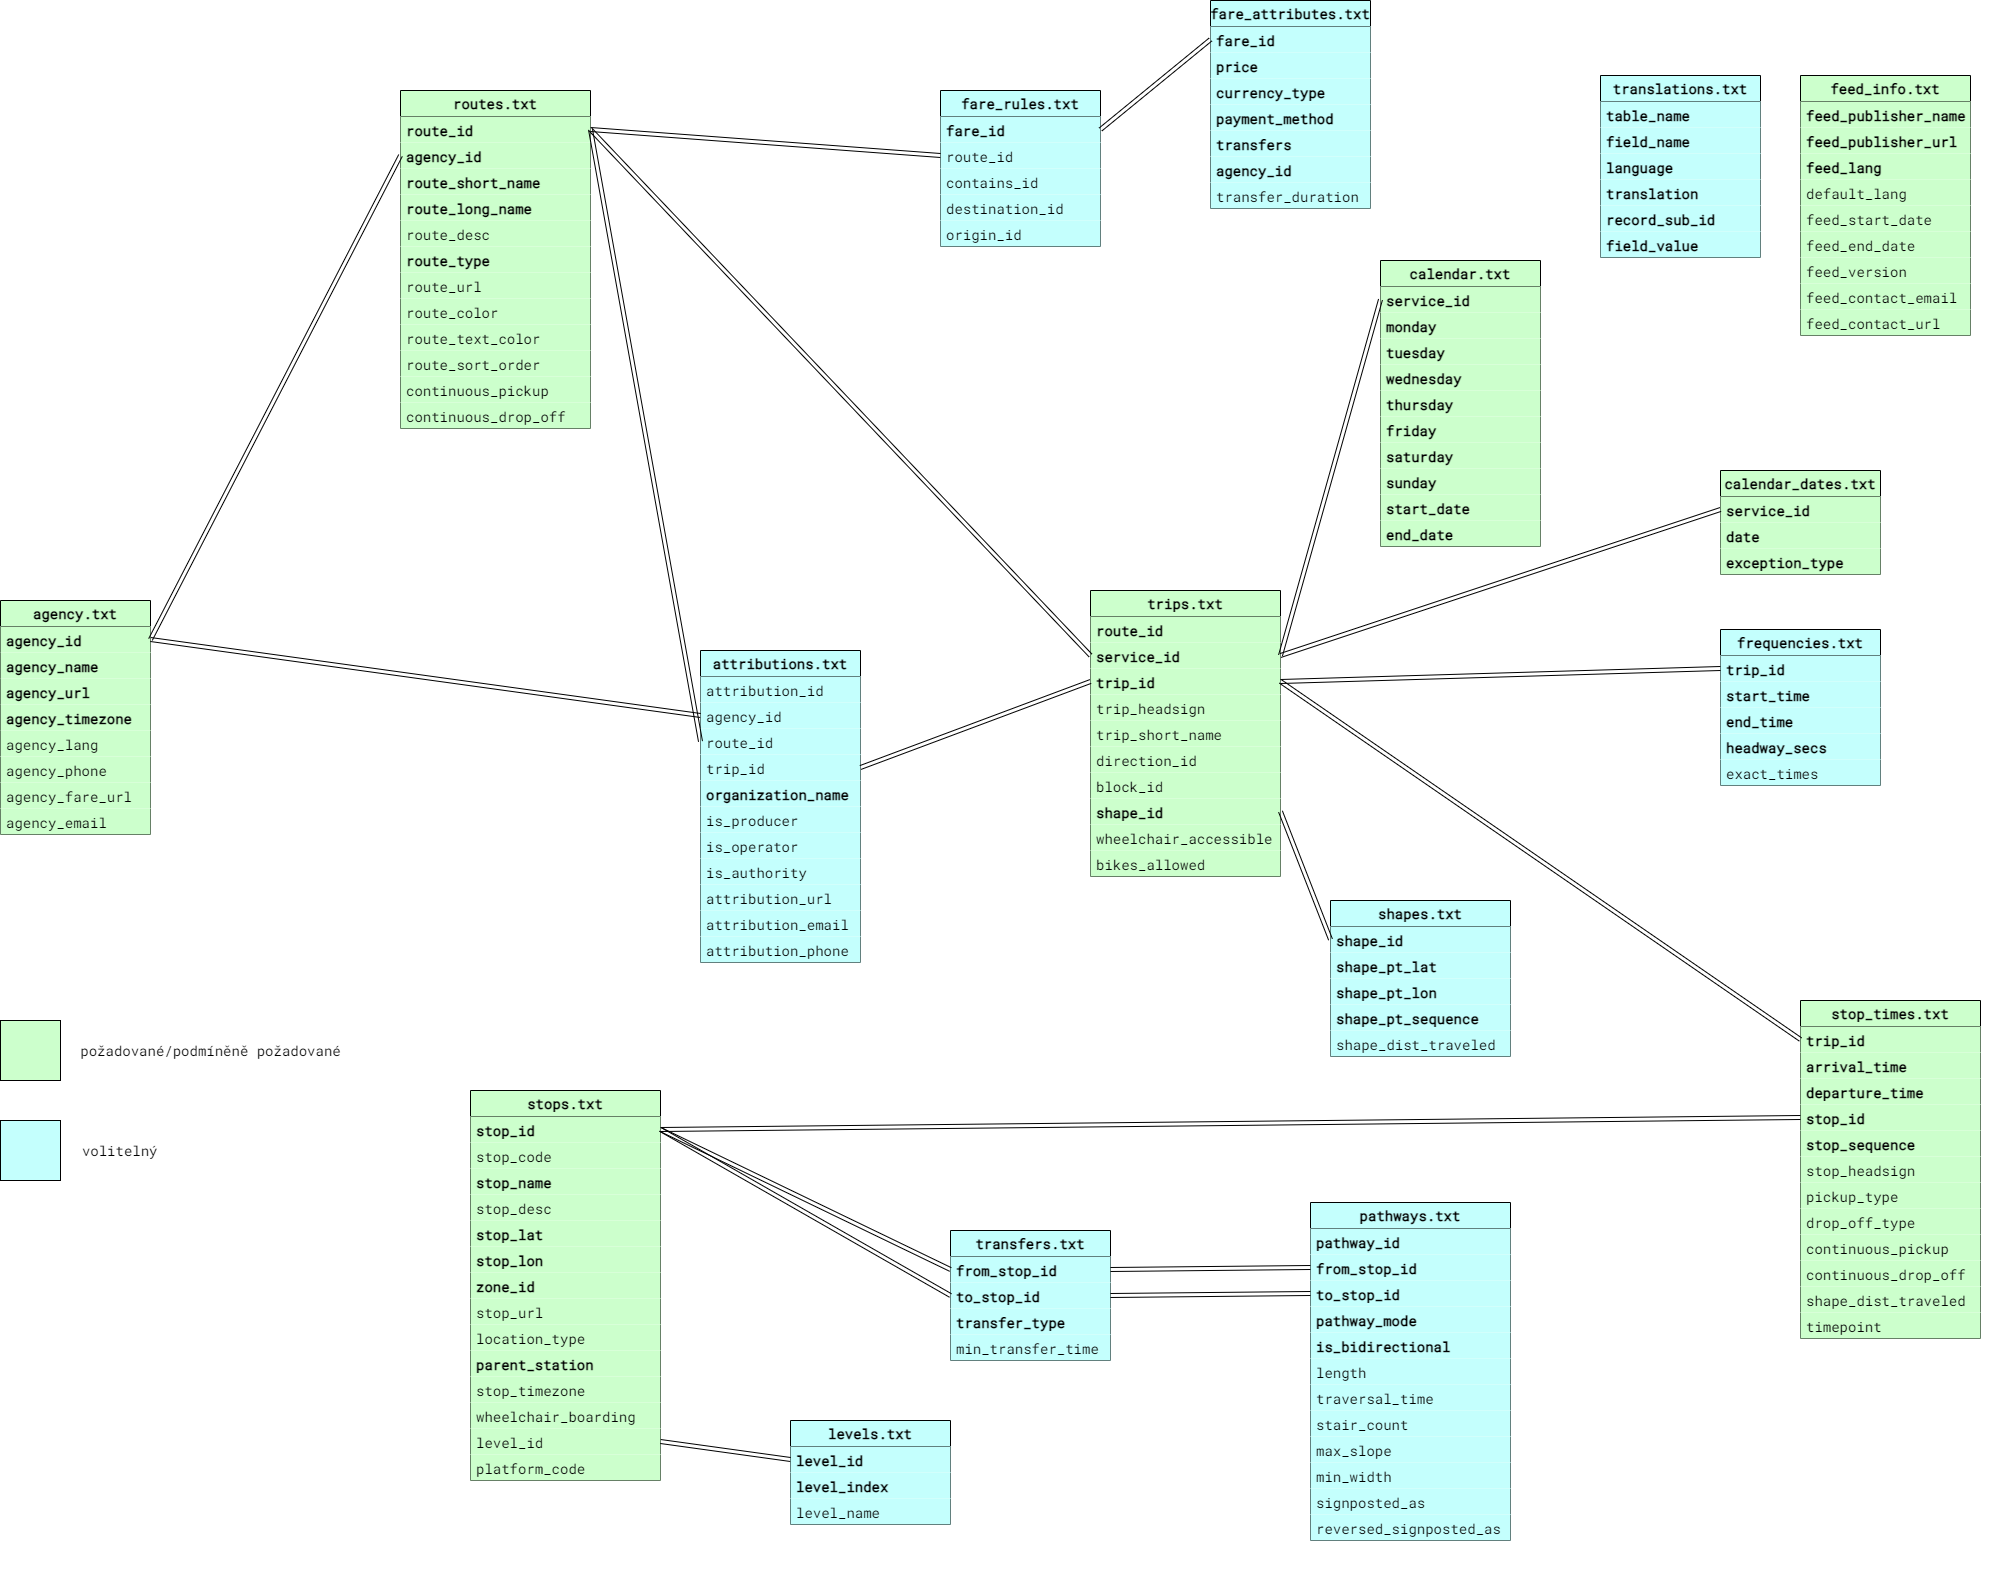
\includegraphics[width=400pt]{./pictures/GTFS-diagram.PNG}
    \caption[Diagram GTFS datasetu]{Diagram GTFS datasetu}
	\label{fig:GTFS-diagram}              
\end{figure}

Pro moji diplomovou práci byly dále důležité datové typy jako zeměpisná délka a zeměpisná šířka,
které již podle názvu obsahují zeměpisnou délku a šířku v souřadnicovém systému WGS84, barva zakódovaná 
jako šestimístné hexadecimální číslo, nezáporné číslo s plovoucí desetinnou čárkou a nezáporné celé číslo
nebo enum, což jsou předem definované konstanty.

\subsection{Soubor stops.txt}
\label{stops.txt}
Soubor \textit{stops.txt} se skládá ze 14 polí, z čehož 6 polí je požadovaných nebo podmíněně požadovaných 
a zbytek volitelných. Samotný soubor je požadovaný a měl by se nacházet v každém GTFS datasetu.

Prvním polem je vždy zpravidla \textit{stop\_id}, které je požadované a má datový typ ID.
Tato hodnota jednoznažně určuje každou zastávku. Pro PID\_GTFS, což je GTFS dataset Pražské integrované dopravy,
se pole \textit{stop\_id} skládá z kombinace písmen a čísel v souvislosti s typem spoje.

Druhým polem je volitelné pole \textit{stop\_code} v datovém typu text, což je krátký text nebo číslo, 
které identifikuje lokaci pro řidiče. 

Dalším třetím polem je s datovým typem text \textit{stop\_name}. Jak už název napovídá, tak obsahuje název lokace. 
Je podmíněně požadované kvůli dalšímu volitelnému devátému poli \textit{location\_type} s datovým typem enum, 
které obsahuje druhy lokace.
Toto pole je definováno pomocí čtyř konstant:
\begin{itemize} 
\item 0 nebo prázdné - zastávka nebo nástupiště
\item 1 - železniční stanice 
\item 2 - vchod/východ ze železniční stanice 
\item 3 - místo ve stanici, které neodpovídá s žádnou s ostatní konstantou z \textit{location\_type} 
\item 4 - specifické místo, kde lidé mohou nastoupit/vystoupit z vozidla
\end{itemize}

Čtvrtým polem je volitelné pole \textit{stop\_desc} v textovém datovém typu obsahující popis místa, 
které poskytuje užitečné a kvalitní informace.

Pátým a šestým polem je \textit{stop\_lat} a \textit{stop\_lon} s datovým typem zeměpisná šířka a délka
obsahující přesně tyto dvě hodnoty. Tyto dvě pole jsou podmíněně požadované kvůli poli \textit{location\_type}.

Sedmým polem s datým typem ID je pole \textit{zone\_id}, které je pro tuto diplomovou práci obzvlášť důležité.
Je podmíněně požadované kvůli CSV souboru \textit{fare\_rules.txt}, pokud jsou v něm poskytovány informace o jízdném.
Pokud záznam v CSV souboru \textit{stops.txt} představuje stanici nebo vchod do stanice, je \textit{zone\_id} ignorováno.

Dalším osmým polem je volitelný \textit{stop\_url} s URL adresou na webovou stránku o místě záznamu.

Desátým polem je podmíněně požadované pole \textit{parent\_station} opět kvůli propojení s polem \textit{location\_type}.
Má datový typ ID odkazující na pole \textit{stop\_id} a definuje hierarchii mezi různými místy definovanými v \textit{stops.txt}. 
a obsahuje ID nadřazeného umístění.

Poslední čtyři pole jsou volitelné. Prvním z nich je \textit{stop\_timezone} s datovým typem a zároveň definujícím časové
pásmo, \textit{wheelchair\_boarding} s datovým typem enum, které označuje, zda je z daného místa možné nastupovat na invalidní vozík.
Předposlední je \textit{level\_id} s datovým typem ID odkazující na soubor \textit{levels.txt} definující úroveň
umístění zastávky a poslední je \textit{platform\_code} s datovým typem text, 
což je identifikátor platformy pro zastávku zastávka patřící stanici.

Všechny tyto pole mají pevné pořadí a nesmí se přeházet. Na obrázku \ref{fig:stops} je ukázka CSV souboru \textit{stops.txt}
pro PID\_GTFS dataset, kde nejsou využívány všechny volitelné pole.

\begin{figure}[H] \centering
    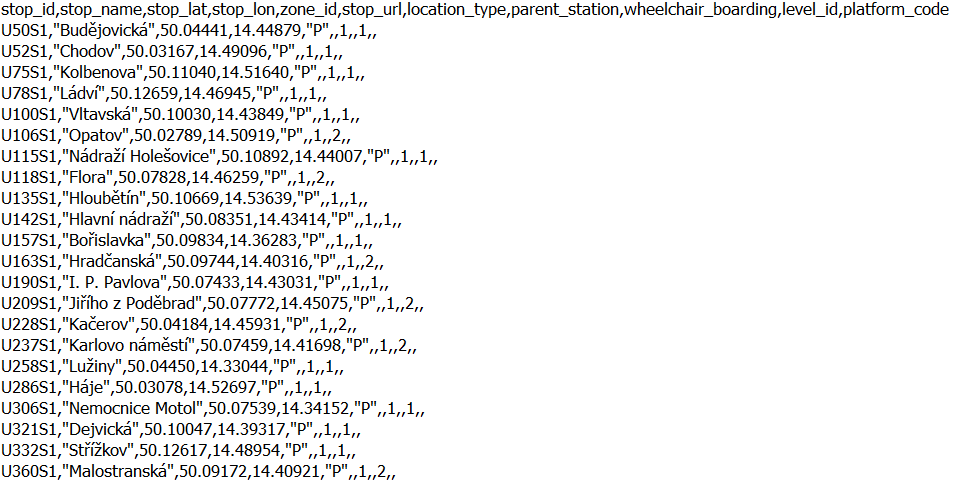
\includegraphics[width=400pt]{./pictures/stops.PNG}
    \caption[Ukázka CSV souboru stops.txt pro PID\_GTFS dataset]{Ukázka CSV souboru stops.txt pro PID\_GTFS dataset}
	\label{fig:stops}              
\end{figure} 